\documentclass{report}
\usepackage{graphicx}
\usepackage{algorithm2e}
\usepackage{geometry}
\usepackage{color}
\geometry{ hmargin=2.5cm, vmargin=2cm } 
\definecolor{title}{rgb}{0.7,0,0}
\definecolor{subtitle}{rgb}{0.5,0,0}
\renewcommand{\thesection}{\arabic{section}}


\begin{document}
\title{Trifocal tensor}
\author{Tifaine CAUMONT and Elisa PRANA}
\maketitle

\tableofcontents
\newpage

\textcolor{title}{\section*{Introduction}}
\addcontentsline{toc}{section}{Introduction} 
The aim of this project was to create an application that enables to establish relations between three pictures. The first step consists in clicking on seven points on each picture representing a 3D scene from different points of view. After seven matches, the program is able to find the position of an element on the third picture if you click on the position of the same element on the two other pictures. 

\textcolor{title}{\section{List of the elements}}

\begin{list}{•}{•}
\item 
Display the help in english with -h : element requested, encoded and working.  
\item
Launch of the program into the console with the name of the three pictures to load : element requested, encoded and working. 
\item
Launch of the program into the console with the name of the three lists to load : element requested, encoded and working. 
\item
Back-up of a list of clicked points : element requested, encoded and working.  
\item
Calculation of a tensor : element requested, encoded and working. 
\item
Transfert pf the points with the tensor : element requested, encoded and working.
\item 
Launch of the program into the console with the path of the repository in which the lists are saved : element not requested, encoded and working.  
\item 
Undo/Redo : element not requested, encoded and but not working.  

\end{list}

\textcolor{title}{\section{Description of the elements encoded}}
\textcolor{subtitle}{\subsection{Tensor}}

A trifocal tensor is a 3x3x3 matrix. It contains 27 elements that we need to calculate. The elements $T_{k}^{il}$ of the tensor have to validate the following expression : 
\begin{center}
 $ \displaystyle { \sum_{k = 1}^{3}} x_{p}^{k}(x_{p}^{'i}x_{p}^{''3}T_{k}^{3l} - x_{p}^{'3}x_{p}^{''3}T_{k}^{il} - x_{p}^{'i}x_{p}^{''l}T_{k}^{33} + x_{p}^{'3}x_{p}^{''l}T_{k}^{i3})$ 
\end{center}
For each point, we have four equations. So in order to have enough equations, we need seven points. 
In order to find the tensor, we have to resolve the following system : $At = 0$, where $A$ is a 28x27 matrix and $t = ( T_{1}^{il}, T_{2}^{il}, T_{3}^{il})$ a vector with 27 components.

\subsubsection{Build $A$}
\paragraph{•}

The first step to resolve the system, is to build the $A$ matrix. Let's call $Ap_{k}^{il}$ the coefficient of the $T_{k}^{il}$ elements in all these equations for the point $p$. We noticed that in each equation, only four tensor coefficients appear. The other are then equal to zero. 

The rows of $A$ correspond to $( Ap_{1}^{il}  Ap_{2}^{il}  Ap_{3}^{il} )$.
For each point, there are four rows in the matrix. The first correponds to $i=1$ and $l=1$, the second to $i=1$ and $l=2$, the third to $i=2$ and $l=1$ and the forth to $i=2$ and $l=2$.

\newpage
Let's take an example with the $p$ point. 
We obtain the four following equations : 
\begin{center}
 $ \displaystyle { \sum_{k = 1}^{3}} x_{p}^{k}(x_{p}^{'1}x_{p}^{''3}T_{k}^{31} - x_{p}^{'3}x_{p}^{''3}T_{k}^{11} - x_{p}^{'1}x_{p}^{''1}T_{k}^{33} + x_{p}^{'3}x_{p}^{''1}T_{k}^{13})$  \textit{with i=1 and l=1}
\end{center}
\begin{center}
 $ \displaystyle { \sum_{k = 1}^{3}} x_{p}^{k}(x_{p}^{'1}x_{p}^{''3}T_{k}^{32} - x_{p}^{'3}x_{p}^{''3}T_{k}^{12} - x_{p}^{'1}x_{p}^{''2}T_{k}^{33} + x_{p}^{'3}x_{p}^{''2}T_{k}^{13})$  \textit{with i=1 and l=2} 
\end{center}
\begin{center}
 $ \displaystyle { \sum_{k = 1}^{3}} x_{p}^{k}(x_{p}^{'2}x_{p}^{''3}T_{k}^{31} - x_{p}^{'3}x_{p}^{''3}T_{k}^{21} - x_{p}^{'2}x_{p}^{''1}T_{k}^{33} + x_{p}^{'3}x_{p}^{''1}T_{k}^{23})$  \textit{with i=2 and l=1} 
\end{center}
\begin{center}
 $ \displaystyle { \sum_{k = 1}^{3}} x_{p}^{k}(x_{p}^{'2}x_{p}^{''3}T_{k}^{32} - x_{p}^{'3}x_{p}^{''3}T_{k}^{22} - x_{p}^{'2}x_{p}^{''2}T_{k}^{33} + x_{p}^{'3}x_{p}^{''2}T_{k}^{23})$  \textit{with i=2 and l=2} 
\end{center}

So in the $A$ matrix, we have the following values for the first equation: 
\begin{center}
$Ap_{k}^{31} = x_{p}^{k}x_{p}^{'1}x_{p}^{''3}$
\end{center}
\begin{center}
$Ap_{k}^{11} = - x_{p}^{k}x_{p}^{'3}x_{p}^{''3}$
\end{center}
\begin{center}
$Ap_{k}^{33} = -x_{p}^{k} x_{p}^{'1}x_{p}^{''1}$
\end{center}
\begin{center}
$Ap_{k}^{13} = x_{p}^{k}x_{p}^{'3}x_{p}^{''1}$
\end{center}

If we adapt this to a general case, we then have  : 
\begin{center}
$Ap_{k}^{3l} = x_{p}^{k}x_{p}^{'i}x_{p}^{''3}$
\end{center}
\begin{center}
$Ap_{k}^{il} = - x_{p}^{k}x_{p}^{'3}x_{p}^{''3}$
\end{center}
\begin{center}
$Ap_{k}^{33} = -x_{p}^{k} x_{p}^{'i}x_{p}^{''l}$
\end{center}
\begin{center}
$Ap_{k}^{i3} = x_{p}^{k}x_{p}^{'3}x_{p}^{''l}$
\end{center}

\paragraph{•}
The issue is now to fill the $A$ matrix in the program. The rows are depending on $p$, $i$ and $l$ and the columns on $k$, $i$ and $l$. Here is the pseudocode to fill the matrix $A$. 

\begin{algorithm}
\SetLine
\caption{Fill the matrix $A$}
\SetLine
Initialize $A$ to 0

\For {p from 0 to 6}{
	\For{i from 0 to 1}{
		\For{l from 0 to 1}{
			\For{k from 0 to 2}{
				$A[4p+2i+l, 9k+3i+l]= -x_{p}^{k}x_{p}^{'3}x_{p}^{''3}$
				
				$A[4p+2i+l, 9k+3i+2]= x_{p}^{k}x_{p}^{'3}x_{p}^{''l}$
				
				$A[4p+2i+l, 9k+6+l]=  x_{p}^{k}x_{p}^{'i}x_{p}^{''3}$
				
				$A[4p+2i+l, 9k+8]= -x_{p}^{k}x_{p}^{'i}x_{p}^{''l}$
				
				increment $k$ of 1
			}
			increment $l$ of 1
		}
		increment $i$ of 1
	}
increment $p$ of 1
}
\end{algorithm}

\newpage
\subsubsection{Calculate T}
Once we have the $A$ matrix, we need to decompose it in $A=UDV^{T}$ with the SVD of the Eigen Library. The $t$ vector is the last column of the $V$ matrix. We can easily pick it up. 
We don't forget to put the element of $t$ in the real tensor $T$ with the right loops: 
\begin{algorithm}
\SetLine
\caption{Calculate $T$}
\SetLine
\For {i from 0 to tensor.getI()}{
	\For{j from 0 tensor.getJ()}{
			\For{k from 0 to tensor.getK()}{
				$T(i,j,k) = t(9*k + 3*i + j))$
				
				increment $k$ of 1
		}
		increment $j$ of 1
	}
increment $i$ of 1
}
\end{algorithm}



\textcolor{subtitle}{\subsection{Transfert}}
The transfert was a difficult part of the project. The main difficulty was to transform the equations into matrices and vectors.

The equation used to transfert the points is the same than the one used for the tensor : 
\begin{center}
 $ \displaystyle { \sum_{k = 1}^{3}} x_{p}^{k}(x_{p}^{'i}x_{p}^{''3}T_{k}^{3l} - x_{p}^{'3}x_{p}^{''3}T_{k}^{il} - x_{p}^{'i}x_{p}^{''l}T_{k}^{33} + x_{p}^{'3}x_{p}^{''l}T_{k}^{i3})$ 
\end{center}

Since we have all the informations about the tensor and two of the three points, the new unknowns are the components of the third point. We decided to put the homogeneous coordinate to 1 in order to simplify the problem. The system to solve is then $Bx=b$ and not $Bx=0$ as we first thought. $B$ is a 4x2 matrix, $x$ a vector of two components and $b$ a vector of four components. 

Let's call $B_{k}^{il}$ the coefficient of $x_{p}^{k}$ depending on what we take for $i$ and $l$. 

We have the four same equations than for the tensor, that we need to rearranged depending of the point transfered.


\subsubsection{Transfert on the first image}
For the first transfert, the colums of $B$ are corresponding to the two coordinates that we search and the line to the different values of i and l. If we remove from the product in the equations the homogeneous coordinate for all the point, we have the following expression for B:

\begin{center}
$B_{k}^{il} = x_{p}^{'i}T_{k}^{3l} - T_{k}^{il} - x_{p}^{'i}x_{p}^{''l}T_{k}^{33} + x_{p}^{''l}T_{k}^{i3}$
\end{center}

The method is the same to find $b$, but we take the coefficient of the homogeneous coordinate and $k=3$ : 

\begin{center}
$b^{il} = x_{p}^{'i}T_{3}^{3l} - T_{3}^{il} - x_{p}^{'i}x_{p}^{''l}T_{3}^{33} + x_{p}^{''l}T_{3}^{i3}$
\end{center}


Here is the pseudocode to build $B$ and $b$ for the first transfert : 
\newpage
\begin{algorithm}
\SetLine
\caption{Build $B$ and $b$}
\SetLine
\For {i from 0 to 1}{
	\For{l from 0 to 1}{
		\For{k from 0 to 2}{

          $ B[2*i + j, k] = x^{'i}T_{2}^{jk} - T_{i}^{jk} - x^{'i}x^{''j}T_{2}^{2k} + x^{''j}T_{i}^{2k}$
          $ b[2*i + j] = - x^{'i}T_{2}^{j2} - T_{i}^{j2} - x^{'i}x^{'j}T_{2}^{22} + x^{''j}T_{i}^{22}$

            increment $k$ of 1
        }    

		increment $l$ of 1
	}
	increment $i$ of 1
}
\end{algorithm}

This time, we applied the SVD with the method solve(b) on the $B$ matrix in order to have $x$. 

\subsubsection{Transfert on the second image}
We take time to understand the fact that the columns of the matrix $B$ were not depending on $k$ anymore, but on $i$ for the second picture and $l$ for the third. Once understood, the method is quite the same. 

We can also write the equation like this : 

\begin{center}
 $ \displaystyle { \sum_{k = 1}^{3}} x_{p}^{k}(x_{p}^{'i} (T_{k}^{3l} - x_{p}^{''l}T_{k}^{33}) + ( x_{p}^{''l}T_{k}^{i3} - T_{k}^{il} ))$
\end{center}

Then we have for $B$ and $b$ :  
\begin{center}
$B_{i}^{il} = x_{p}^{k}(T_{k}^{3l} - x_{p}^{''l}T_{k}^{33})$
\end{center}
\begin{center}
$b^{il} = x_{p}^{k}(x_{p}^{''l}T_{k}^{i3} - T_{k}^{il})$
\end{center}

Since there is the $x_{p}^{k}$ element, we need to have a sum in the loop. Here is the pseudocode:

\begin{algorithm}
\SetLine
\caption{transfert to the second image}
\SetLine
\For {i from 0 to 1}{
	\For{j from 0 to 1}{
		\For{k from 0 to 2}	{ 
        $B[2*i + j, i] += x^{k}(T_{2}^{jk} - x^{''j}T_{2}^{2k})$
        
        $b[2*i + j] += x^{k}(-x^{''j}T_{i}^{2k} + T_{i}^{jk})$

		increment $k$ of 1
		}
		increment $j$ of 1
	}
	increment $i$ of 1
}
\end{algorithm}
We apply the SVD with the method solve(b) on the $B$ matrix in order to get $x$.

\newpage 
\begin{figure}[ht]
   \begin{center}
	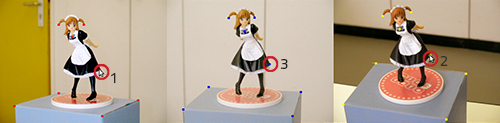
\includegraphics[width=0.8\textwidth]{Tenseur.png}
	\caption{Transfert on the second image after clicking on the first and the third images.}
	\label{fig:mon image}
	\end{center}
\end{figure}

\subsubsection{Transfert on the third image}
The method is similar to the one for the third transfert.
The equation can be written like this : 

\begin{center}
 $ \displaystyle { \sum_{k = 1}^{3}} x_{p}^{k}(x_{p}^{''l}(T_{k}^{i3} - x_{p}^{'i}T_{k}^{33}) + ( x_{p}^{'i}T_{k}^{3l} - T_{k}^{il}))$ 
\end{center}

Then we have for $B$ and $b$ :  
\begin{center}
$B_{l}^{il} = x_{p}^{k}(T_{k}^{i3} - x_{p}^{'i}T_{k}^{33})$
\end{center}
\begin{center}
$b^{il} = x_{p}^{k}(x_{p}^{'i}T_{k}^{3l} - T_{k}^{il})$
\end{center}

Here is the pseudocode : 
\begin{algorithm}
\SetLine
\caption{transfert to the third image}
\SetLine
\For {i from 0 to 1}{
	\For{j from 0 to 1}{
		\For{k from 0 to 2}	{ 
		$B[2*i + j, j]$ +=  $ x^{k}T_{i}^{2k} -x^{''i}T_{2}^{2k})$
		
        $b[2*i + j]$ += $x^{k}(T_{i}^{jk} -x^{'i}T_{2}^{jk} )$

		increment $k$ of 1
		}
		increment $j$ of 1
	}
	increment $i$ of 1
}
\end{algorithm}
\subsubsection{Use the right transfert}
Once the transfert working for three pictures, we had to put conditions on the click event to calculate the right transfert, depending on the two first points clicked.  

 
\textcolor{subtitle}{\subsection{Saving the clicked points}}
At first, the lists were lists of 7 points and when clicking, the first point of the list was changed. It was not a great idea. 
Then we add an eighth point, calculated with the transfert in order to keep the list of the seven points needed to build the tensor. The problem was that we did not save all the points and we were writting in the files with std::ifstream. So we changed the saveMatrix function in order to save as many points as wanted. But it still changed the initial file. 
We decided to save the point int tmp/list.list with a new method : $" << "$. A row is just added into the matrix and the file saved for each click. 
Finally, we created a function (updateMatrix) in order to do the resizing of the matrix and the saving in a file. 

\textcolor{subtitle}{\subsection{Save or load a list in a file}}
\subsubsection{Saving}
At the beginning, the lists of the clicked points were saved in the initial file. This was a probleme since the user may not want to modify his files. 
So we decided to save them directly into the repository tmp/.
Finally, we had an option for the user. He can specify a repository when he launches the program. The lists are then saved in this repository. 

All the files are saved with the format ask in the subject (row and col at the beginning). In order to do that, we activated the header to true in saveMatrix()in mathIO. 

\subsubsection{Loading}
The lists are loaded at the beginning of the program, according to the options that the user chooses. In order to manage the empty list or the list containing a row or column equal to zero, we modified the function loadMatrix() and readMatrixHeader() in mathIO. 

\textcolor{subtitle}{\subsection{Launch the program with arguments}}
We have done a program which can be launched with or without arguments. When the program is launched, there is a test that checks if there are some arguments, and how many. With $argc$, we have the number of arguments written in the command, and with $argv[i]$, we can pick up the argument to use it in a fonction for example.
Be careful to not forget that when we wrote for example ./bin/trifocal, it counts like an argument.
When the user does not give arguments, the default program is executed. It's a program with the three default images, and the three default lists with already the seven points in it.
\paragraph{•}
\begin{center}
\begin{figure}[ht]
    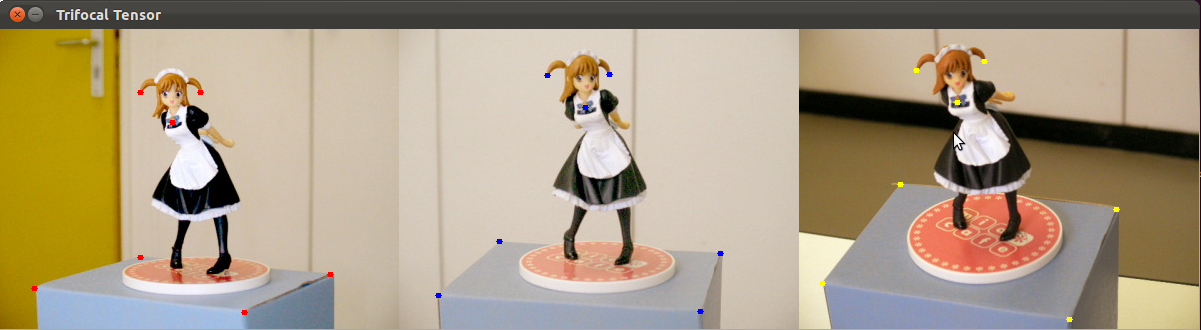
\includegraphics[scale=0.4]{defaut.png}
    \caption{Program launched without arguments}
    \label{Picture 1}
\end{figure} 
\end{center}

\paragraph{•}
If the user wants, he can give three more arguments, which are the three images he wants to load. If he loads some images, there will be no list with points. He has to clic the corresponding points on the three images. 

\newpage
\begin{center}
\begin{figure}[ht]
    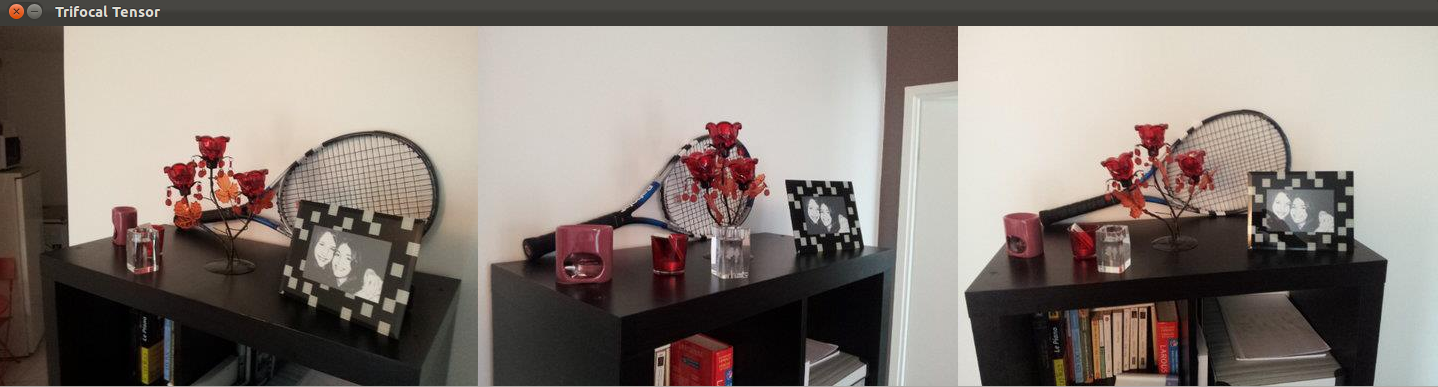
\includegraphics[scale=0.334]{images.png}
    \caption{Program launch with user's pictures}
    \label{Picture 2}
\end{figure} 
\end{center}

\paragraph{•}
If the user wants to have his own images and lists of points, he can give six arguments, first the three images, then the three lists. 
The user can also specify the path of the repository in which he wants the list to be saved, when he gives some arguments. 

\textcolor{subtitle}{\subsection{Undo/Redo}}
We wanted to make undo-redo in the program because currently, if you click a wrong point, you have to start again from the beginning if you don't want to modify the files. In order to do that, we created an undo function that delete the last point. We succeed in modifying the last point clicked of the last list modified. This function is working, the point disappear of the list, but it is still displayed on the screen. 
So we did not go further. The code is in commentary in the files. 

\textcolor{title}{\section{Improvement}}
This program can still be improved. 

\textcolor{subtitle}{\subsection{Resize }}
Currently, when we load pictures which are to big, the program works but does not adapt the size of the images to the size of the screen. So we can't see them on our screen and work with it. 
We want to resize these pictures in order to have a window contained in the screen surface. 

\textcolor{subtitle}{\subsection{Zoom}}
When we don't load a list of point, launching the program, we have to click on the seven matching points to calculate the tensor and use the transfert. But it is difficult to click precisely. So we thought about creating a zoom with SDL rotozoom. We did not had time to implement it, but it is a way to click without to much error.

\textcolor{subtitle}{\subsection{Options}}
The options in the console are working, but are not very precised. We still can work on it in order to manage all the configuration that the user may use. 

\textcolor{subtitle}{\subsection{Undo/Redo}}
As the undo function is not displayed, we can improve the project with a functionnal undo/redo function. We could delete the points clicked and redo them in case of error. This function is very used in all the programs and enable a better user experience. 

\newpage
\textcolor{title}{\section*{Conclusion}}
\addcontentsline{toc}{section}{Conclusion} 
This project was quite absorbing since he will never be completely finished. Actually, the tricky part was to pass from mathematics function to code. Using the Eigen Library, it forced us to search the functions we could use in the documentation. We learn to work with code that is not ours and not explained by someone. 



We decided to write all the project in english in order to pratice. We usually use english name for our functions so we can also write the commentaries in english. 

Even if we did not success in implementing all the functions we wanted, the program is functionnal and the transferts are working. 

\end{document}
